
\chapter{Proposed Framework}
\label{capitulo4}


\section{Proposals}

\subsection{One camera with object calibration}
\begin{figure}[H]
\centering
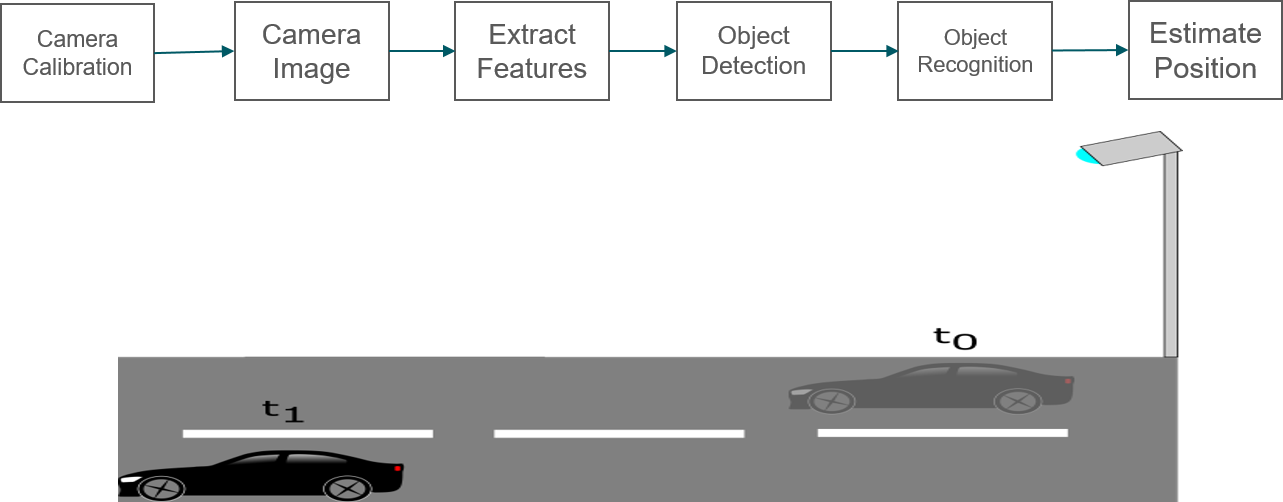
\includegraphics[width=\textwidth]{imagens/proposal1.png}
\caption{Proposal using only one camera with object calibration, this firts approach is based on \cite{8678911}}
\label{fig:proposal1}
\end{figure}


\subsection{Proposal 2 – One camera with known map}
\begin{figure}[H]
\centering
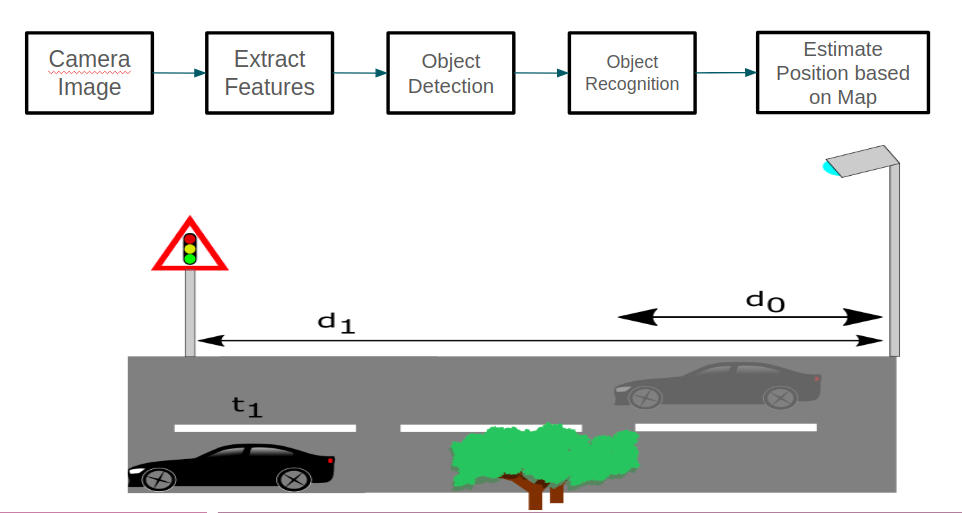
\includegraphics[width=\textwidth]{imagens/proposal2.png}
\caption{Proposal using Proposal 2 – One camera with known map}
\label{fig:proposal2}
\end{figure}


\subsection{Proposal 3 – Multicameras}
\begin{figure}[H]
\centering
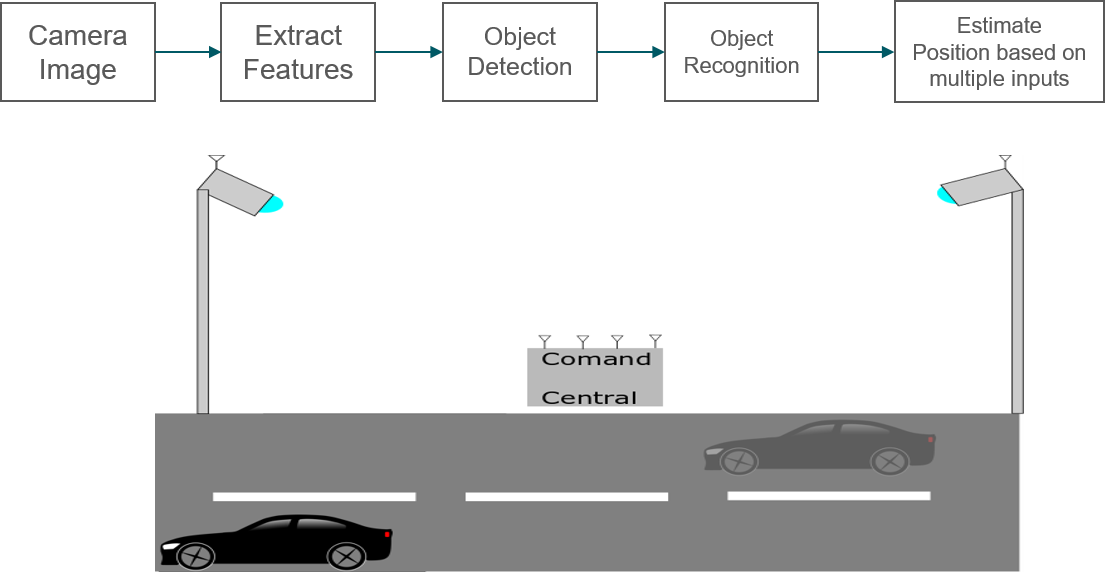
\includegraphics[width=\textwidth]{imagens/proposal3.png}
\caption{Proposal using multicameras}
\label{fig:proposal3}
\end{figure}



\section{Inverse Perspective Mapping }
Inverse perspective mapping is a mathematical technique that remove the effects of distortion of a picture when transforming the perspective of the image to another perspective. In spite of disparity mapping, inverse perspective mapping method requires only one camera and this method cannot provide depth information directly ~\cite{Tuohy2010}.

Camera must be located in front of the car with an angle of \(\theta\) to down. Figure \ref{fig:ImageRelationSystem} shows the setup.

\begin{figure}[h]
\centering
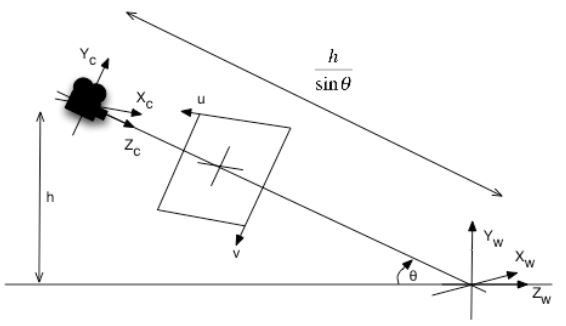
\includegraphics[scale=0.5]{imagens/Inverse Perspective Mapping.JPG}
\caption{Image coordinate system in relation to world coordinate
system.}
\label{fig:ImageRelationSystem}
\end{figure}
\par


This setup was selected based on solution of \cite{Wongsaree2018}, the mathematical background is to create top-down view, the surface road point is known as $(X_w,Y_w,Z_w)$
that projects to the image plane $(u,v)$ is a must. As disrupted in Figure \ref{fig:ImageRelationSystem}. For rotatation angle $(\theta)$, which is angle between camera and the surface, the IPM equation is based on \cite{7759904} and is shown is Equation \ref{eq:eq1}:

\begin{equation}
    (u,v,1)^T = K\cdot T \cdot K (X_w,Y_w, Z_w,1)^T
    \label{eq:eq1}
\end{equation}

where R is the rotation matrix given in the equation \ref{exp2}.
\begin{equation} \label{exp2}
R=
\begin{bmatrix}
1 & 0 & 0 & 0\\
0 & \cos{\theta} & -\sin{\theta} & 0\\
0 & \sin{\theta} & \cos{\theta} & 0\\
0 & 0 & 0 & 1
\end{bmatrix}
\end{equation}
\par

T is the translation matrix given in the equation \ref{exp3}. Where h means the height of the position of the camera.
\begin{equation} \label{exp3}
T=
\begin{bmatrix}
1 & 0 & 0 & 0\\
0 & 1 & 0 & 0\\
0 & 0 & 1 & \frac{-h}{\sin{\theta}}\\
0 & 0 & 0 & 1
\end{bmatrix}
\end{equation}


\par
K is the camera parameter matrix given in the Equation \ref{exp4}. Where $f$ is the focal length of the camera, $s$ is the skew parameter and $u_0, v_0$ are the center of the pixel of desired image size. 
\begin{equation} \label{exp4}
K =
\begin{bmatrix}
f & s & u_0 & 0\\
0 & f & v_0 & 0\\
0 & 0 & 1 & 0\\
\end{bmatrix}
\end{equation}

The Equation \ref{exp4} can be replaced using the real parameters of this test scenario and these parameters are $f = 2.92 mm, s=0, u_0=240, v_0=160$. Replacing the Equations \ref{exp2},\ref{exp3}, \ref{exp4} into the initial Equation \ref{eq:eq1}, achieving the new Equation \ref{eq:eq2}.

\begin{equation}
    \begin{bmatrix}
u\\ 
v\\ 
1
\end{bmatrix}
=\begin{bmatrix}
P_{11} & P_{12} & P_{13} & P_{14}\\ 
P_{21} & P_{22} & P_{23} & P_{24}\\ 
P_{31} & P_{32} & P_{33} & P_{34}
\end{bmatrix}
\begin{bmatrix}
X_w\\ 
Y_w\\ 
Z_w\\
1
\end{bmatrix}
\label{eq:eq2}
\end{equation}

where the matrix P was gotten from product between K, T, and R. As is only necessary to evaluate the position of the road, so the coordinate $Y_w$ can be equal to 0, so simplifying the Equation \ref{eq:eq2}, so it is given by Equation \ref{eq:eq3}.

\begin{equation}
    \label{eq:eq3}
    \begin{bmatrix}
u\\ 
v\\ 
1
\end{bmatrix}
=\begin{bmatrix}
P_{11} & P_{12}  & P_{14}\\ 
P_{21} & P_{22}  & P_{24}\\ 
P_{31} & P_{32}  & P_{34}
\end{bmatrix}
\begin{bmatrix}
X_w\\ 
Z_w\\
1
\end{bmatrix}
\end{equation}

Based on the Equations above, it is possible to infer the Equation \ref{eq:eq4} for compute the distance from the camera until the object. 

\begin{enumerate}
    \item Calculating average intensity in row direction from bottom row up to top row
    \item The average intensity of each row is compared with the threshold level (obtained from the experimental) which is 50. The starting position of an object is indicated if the average intensity in that row is greater than 50 and the order of that row is stored in a parameter p.
    \item The distance between object and vehicle is therefore calculated using a linear equation given in \ref{eq:eq4}.
\end{enumerate}

\begin{equation}
    \label{eq:eq4}
    d = ap+b
\end{equation}

where $d$ is distance between camera and object and vehicle in meter, $p$ is the order of the row that object is detected and $a, b$ are constants.

 
\section{Framework Architecture} 

\begin{figure}[H]
\centering
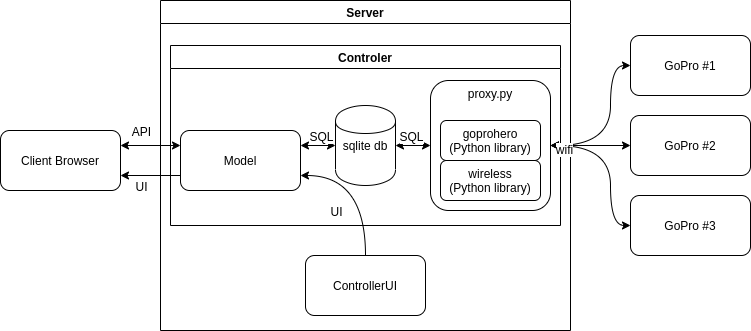
\includegraphics[scale=0.6]{imagens/diagram.png}
\caption{Architecture approach of framework}
\label{fig:framework}
\end{figure}

\begin{figure}[H]
\centering
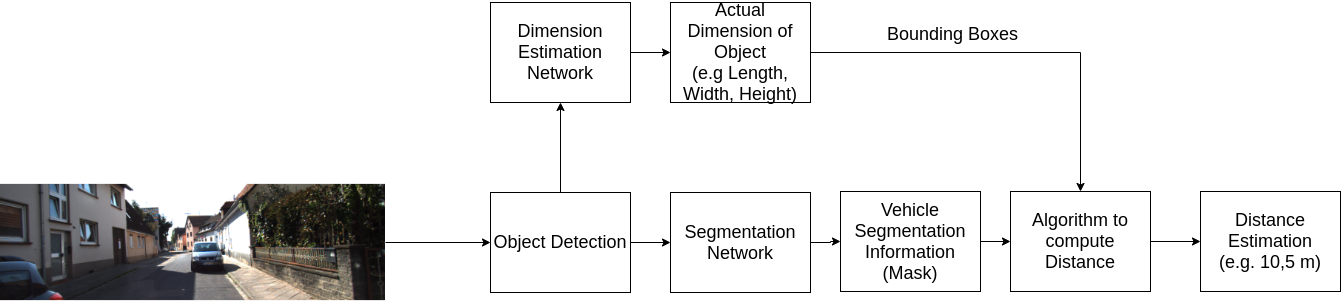
\includegraphics[width=\textwidth]{imagens/Network Behavior.png}
\caption{Architecture approach of framework}
\label{fig:networkBehavior}
\end{figure}